\chapter{SLA - Lightly cluttered room}
\label{app:sla}

Each figure in this appendix shows the distance between the tag real position and the tag estimated position by the \gls{sla}. Each simulation has been made in the same room, the room in Fig. \ref{fig:room_cluttered} with the blue furniture. The anchor has been set at different position for each simulation. 

\subsubsection*{Anchor in a corner}

\begin{figure}[H]
\centering
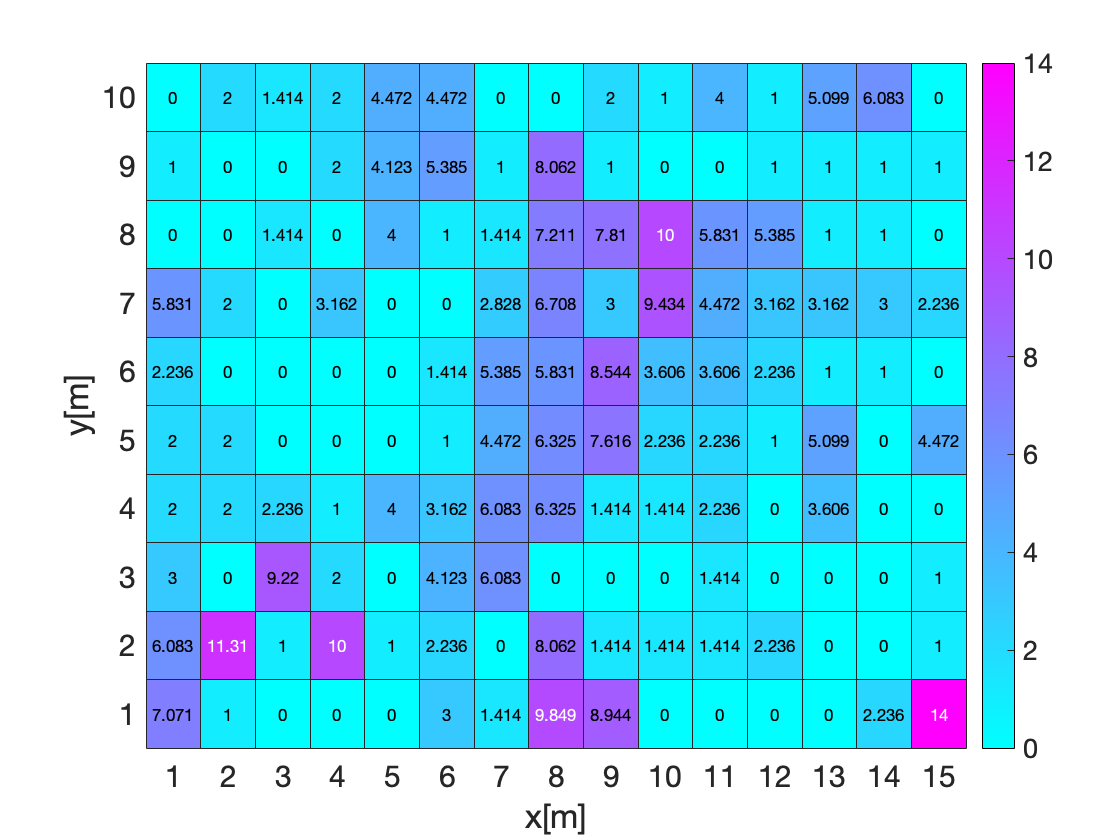
\includegraphics[width=.9\linewidth]{Images/Anchor_at_(3_9).png}
\caption{Anchor located at (3, 9).}
\end{figure}

\begin{figure}[H]
\centering
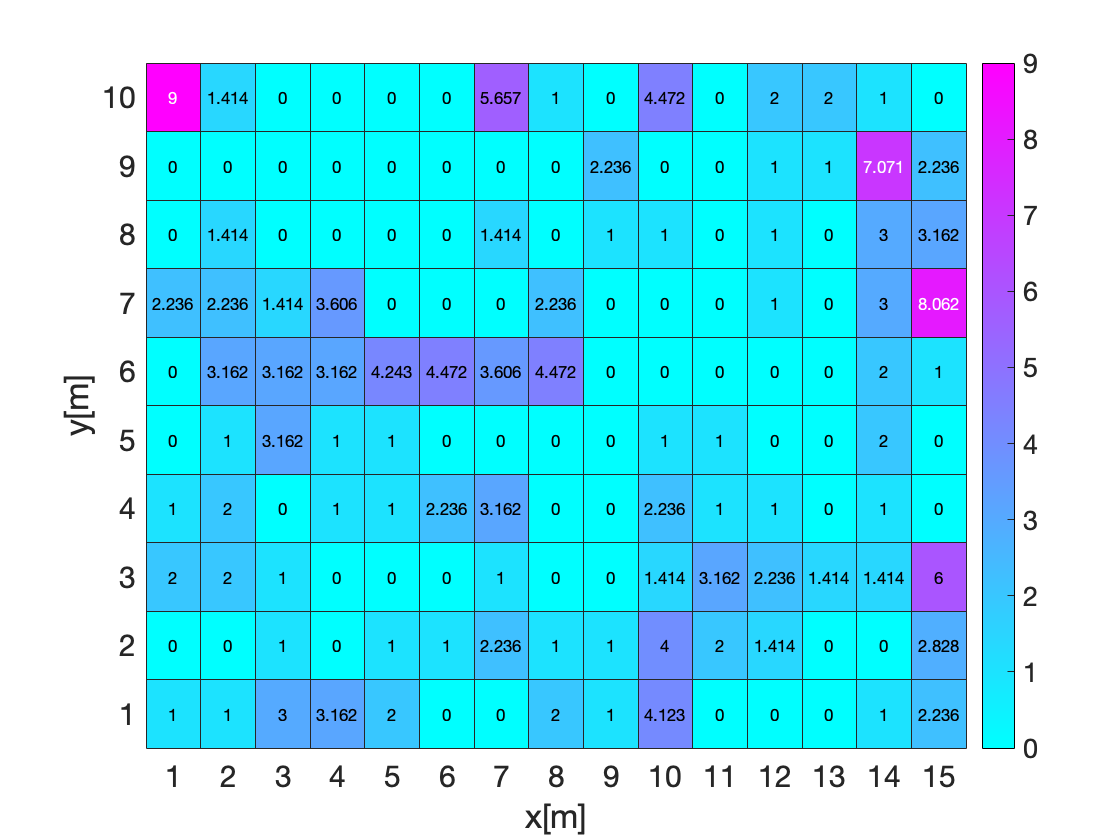
\includegraphics[width=.9\linewidth]{Images/Anchor_at_(12_1).png}
\caption{Anchor located at (12, 1).}
\end{figure}

\begin{figure}[H]
\centering
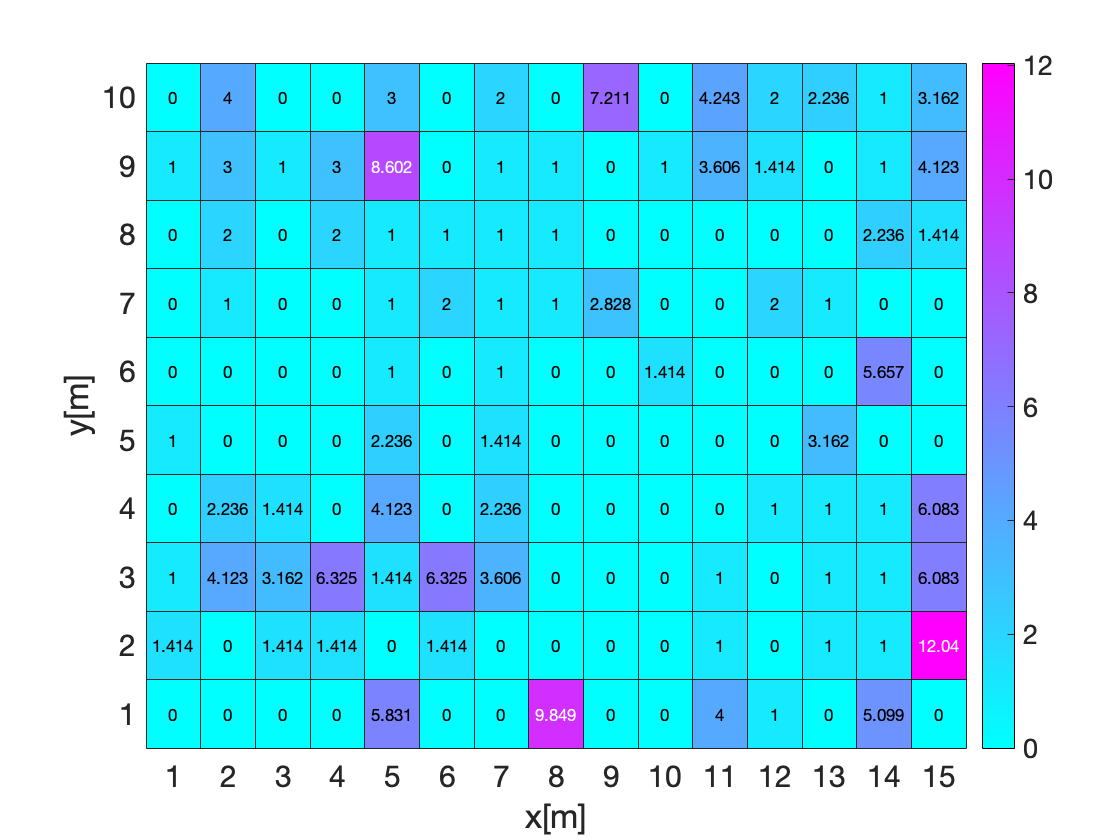
\includegraphics[width=.9\linewidth]{Images/Anchor_at_(13_9).png}
\caption{Anchor located at (13, 9).}
\end{figure}

\begin{figure}[H]
\centering
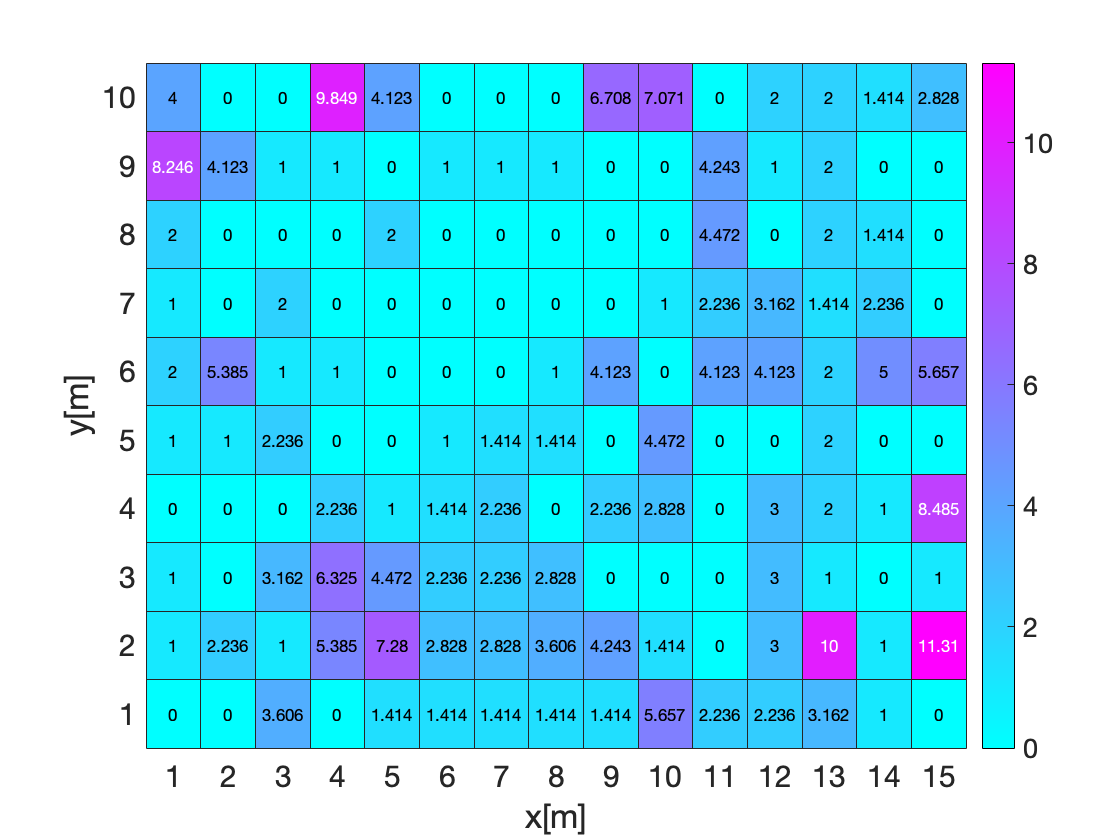
\includegraphics[width=.9\linewidth]{Images/Anchor_at_(14_9).png}
\caption{Anchor located at (14, 9).}
\end{figure}

\subsubsection*{Anchor in the middle of a wall}

\begin{figure}[H]
\centering
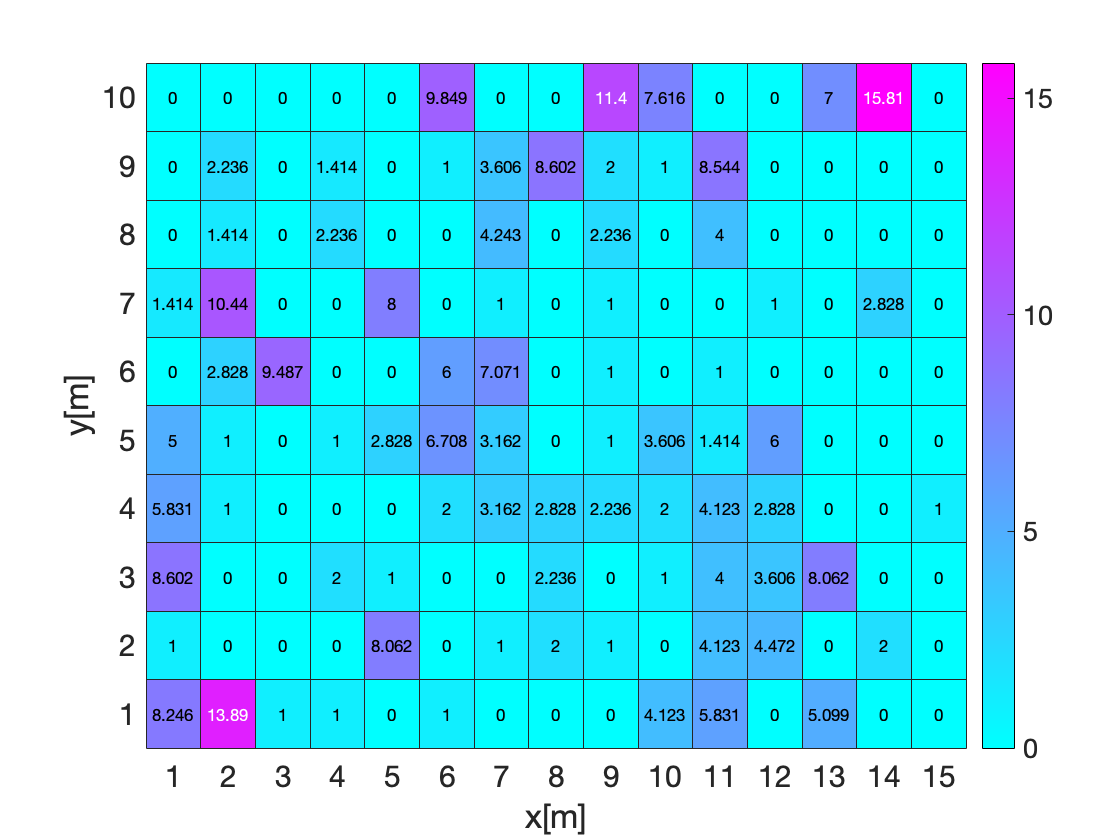
\includegraphics[width=.9\linewidth]{Images/Anchor_at_(9_3).png}
\caption{Anchor located at (9, 3).}
\end{figure}

\begin{figure}[H]
\centering
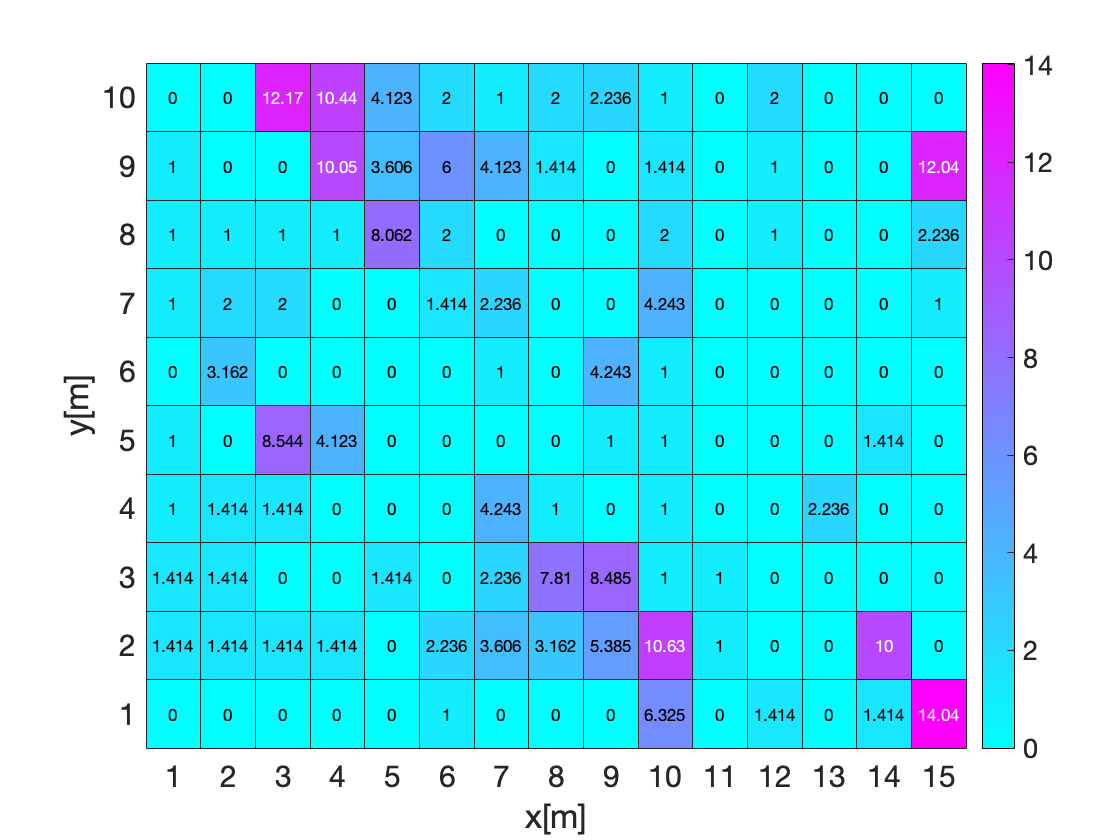
\includegraphics[width=.9\linewidth]{Images/Anchor_at_(9_9).png}
\caption{Anchor located at (9, 9).}
\end{figure}

\begin{figure}[H]
\centering
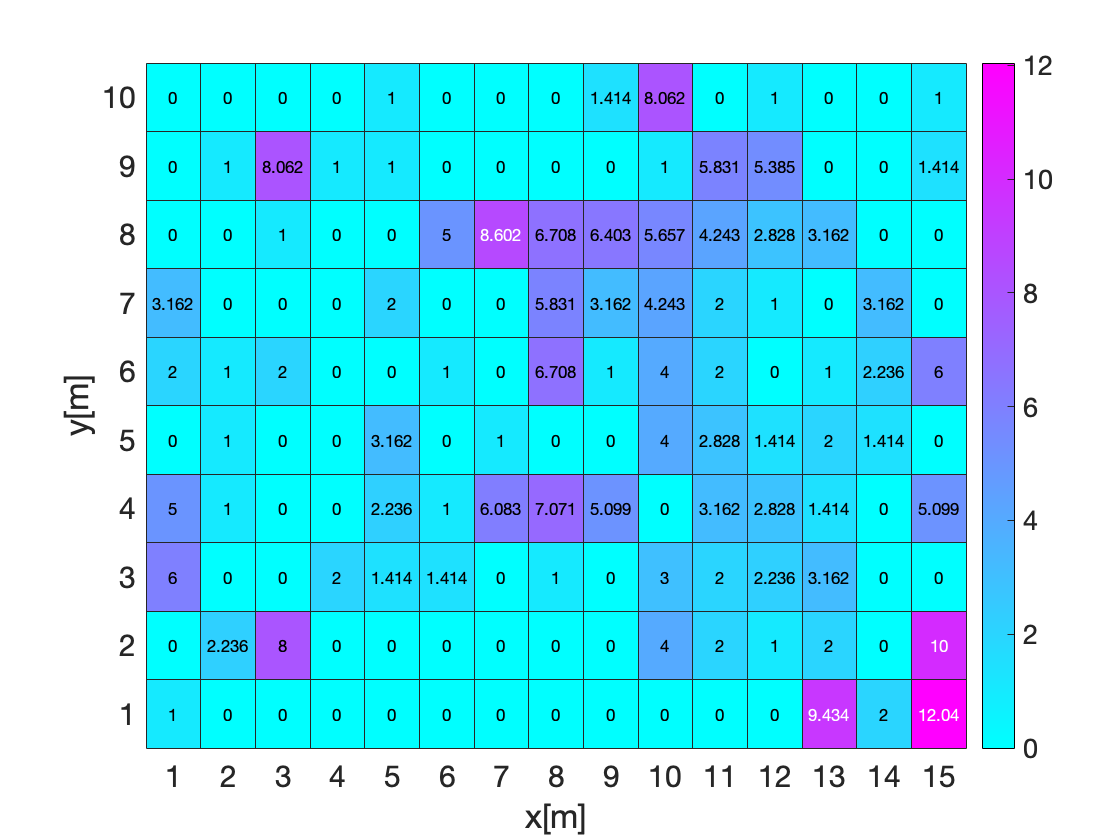
\includegraphics[width=.9\linewidth]{Images/Anchor_at_(12_6).png}
\caption{Anchor located at (12, 6).}
\end{figure}

\subsubsection*{Anchor in the middle of the room}

\begin{figure}[H]
\centering
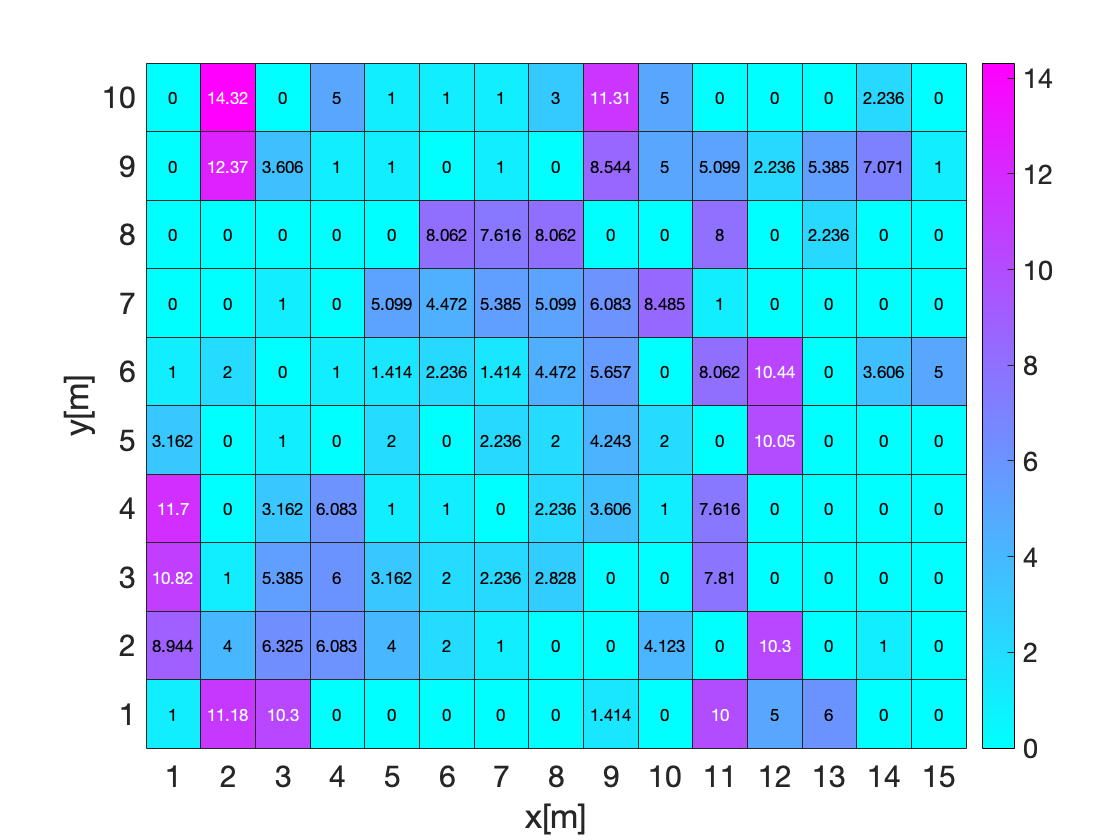
\includegraphics[width=.9\linewidth]{Images/Anchor_at_(7_4).png}
\caption{Anchor located at (7, 4).}
\end{figure}

\begin{figure}[H]
\centering
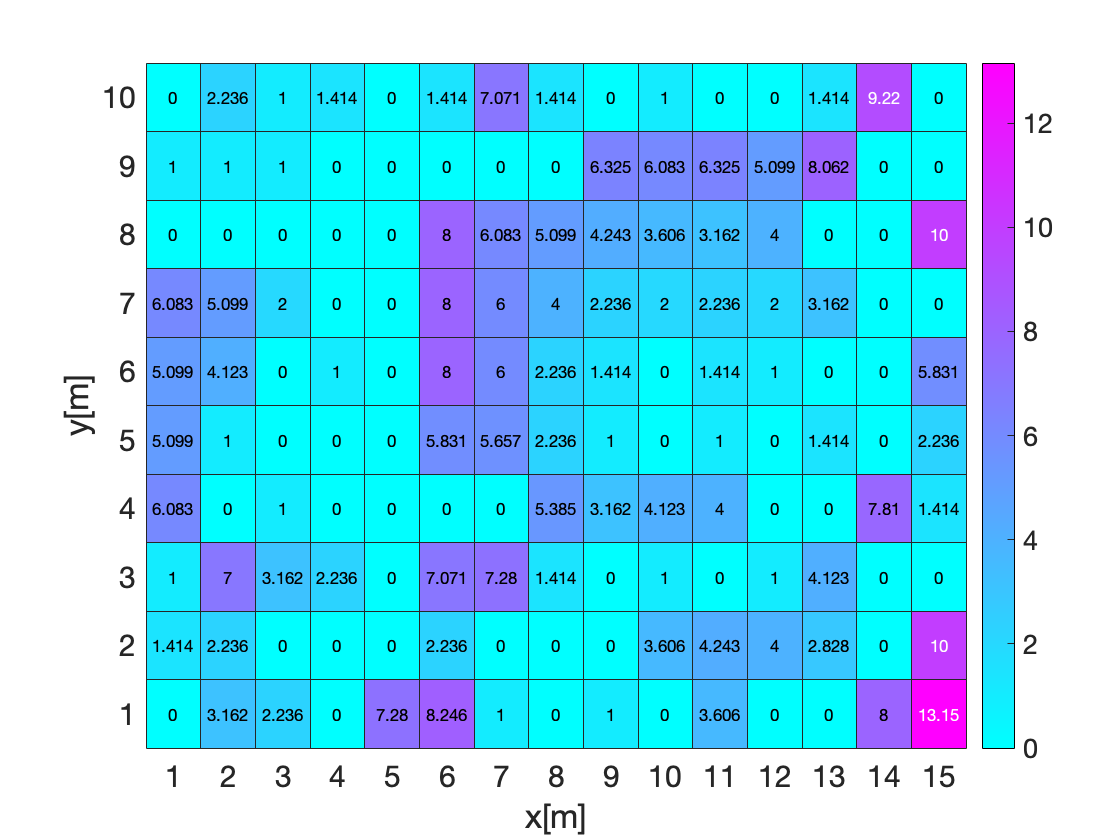
\includegraphics[width=.9\linewidth]{Images/Anchor_at_(10_6).png}
\caption{Anchor located at (10, 6).}
\end{figure}


